\chapter{Results and Observations}

\section{Tobamovirus Data}
For the Tobamovirus data we can see that the projection \ref{T1} of the complete data obtained using standard PCA gives three sub-groups. Then we have \ref{T2} which is the projection obtained using PPCA closed form given in []. Figure \ref{T3} is the projection obtained by the PPCA run with EM algorithm. The projection is the same except for being rotated about some point. The roation is dependent on the initialization of the algorithm.\\\\
For the missing data case (20\% missing), it is clear that both figure \ref{T4} and \ref{T5} is able to obtain three sub-grounps. The salient features of the projection  is clear, even when all data points have suffered from at least one missing value. Both the algorithms seems to perform equally good in this dataset.
\begin{figure}
	\centering
  	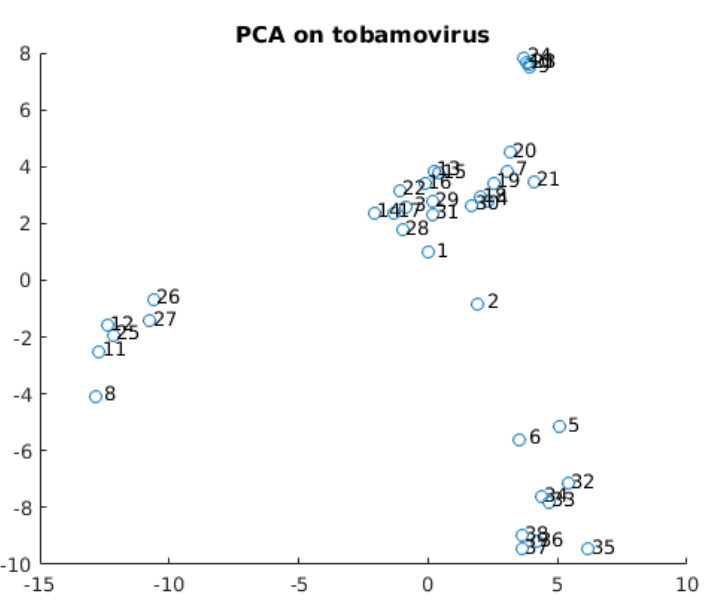
\includegraphics[width=1.0\textwidth]{./images/PCA.png}
  	\caption{Standard PCA}
  	\label{T1}
\end{figure}

\begin{figure}
	\centering
  	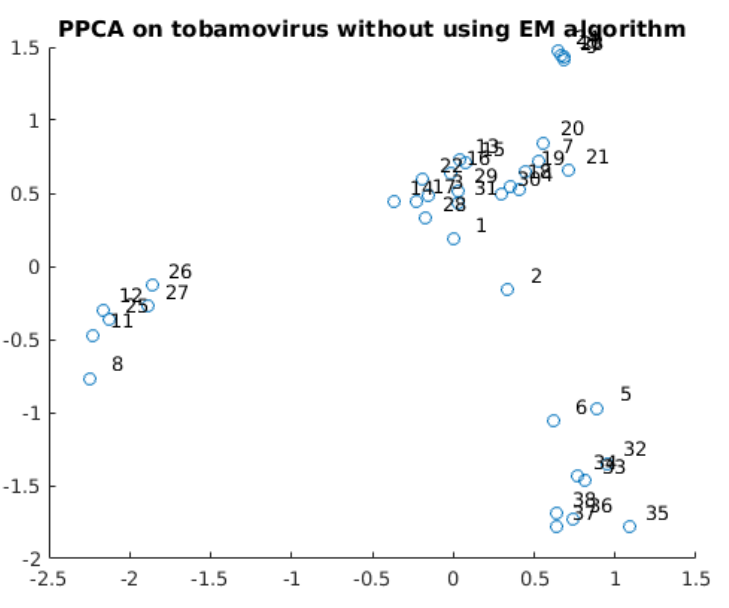
\includegraphics[width=0.7\textwidth]{./images/PPCA.png}
  	\caption{PPCA using closed form formula}
  	\label{T2}
\end{figure}

\begin{figure}
	\centering
  	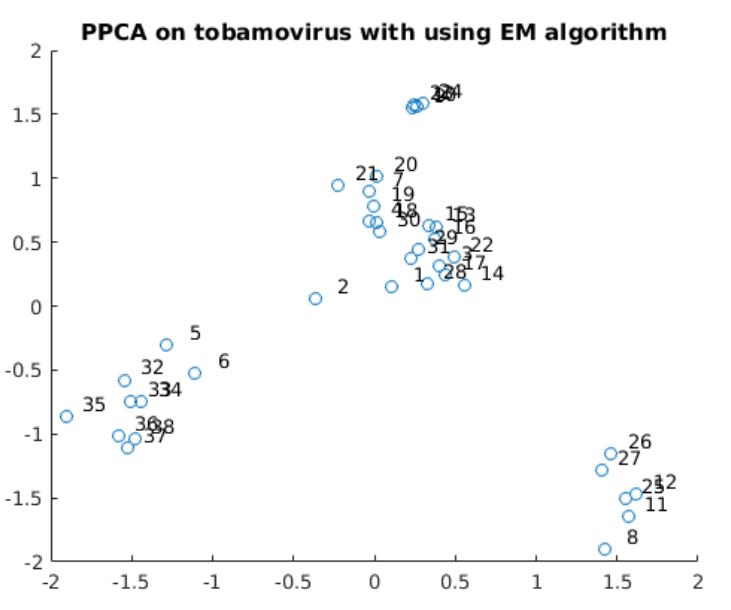
\includegraphics[width=0.7\textwidth]{./images/PPCAEM.png}
  	\caption{PPCA using EM algorithm}
  	\label{T3}
\end{figure}

\begin{figure}
	\centering
  	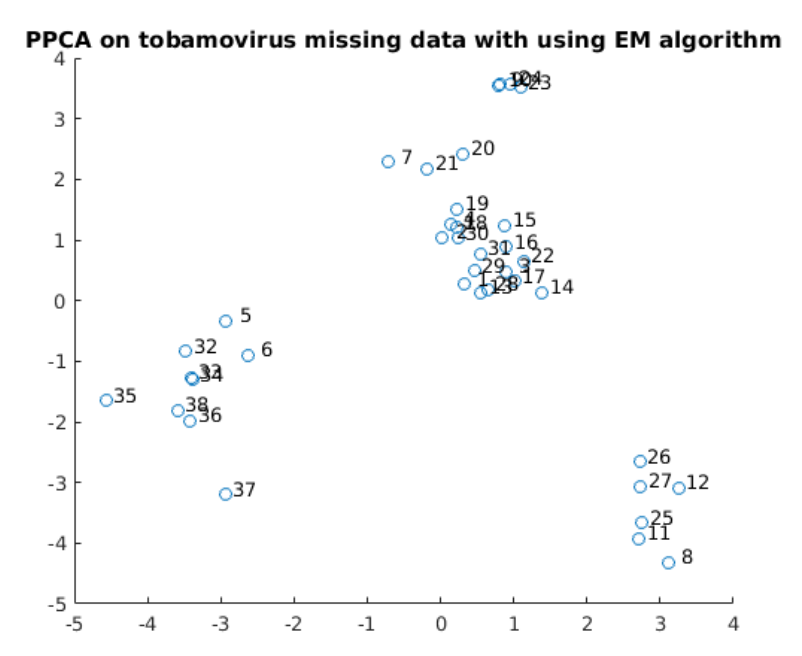
\includegraphics[width=0.7\textwidth]{./images/PPCAEMMiss.png}
  	\caption{PPCA projection with 20\% missing data using EM}
  	\label{T4}
\end{figure}

\begin{figure}
\centering
  	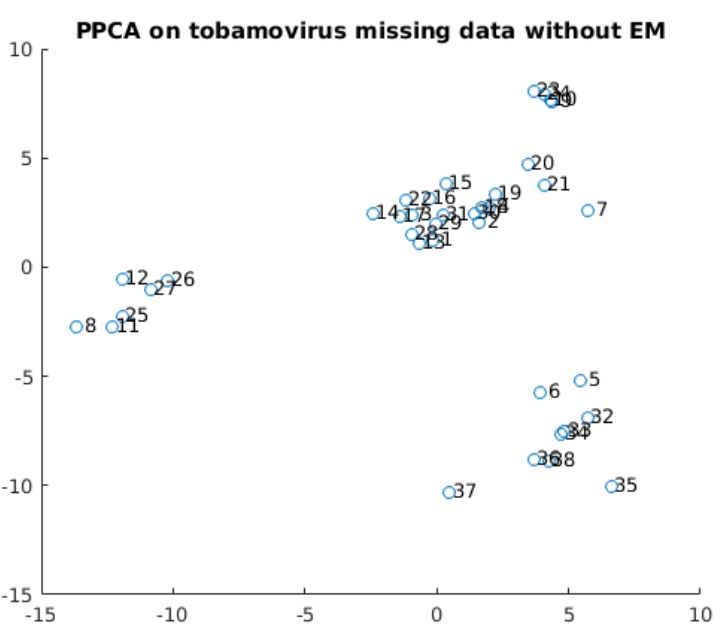
\includegraphics[width=0.7\textwidth]{./images/PCAMiss.png}
  	\caption{PCA projection with 20\% missing data}
  	\label{T5}
\end{figure}

\newpage

\section{MNIST Data}

MNIST data contains $28\times 28$ images. Each images contains a handwritten digit. The task is predition of the digits. The experiment design outlines in the last chapter is followed. \\\\
The plot \ref{T6} shows how the accuracy increases rapidly at start but then becomes static. The latent dimension $k=133$ is a good choice as it has highest accuracy in the region plotted and also the increase becomes very less after that point.\\

\begin{figure}
\centering
  	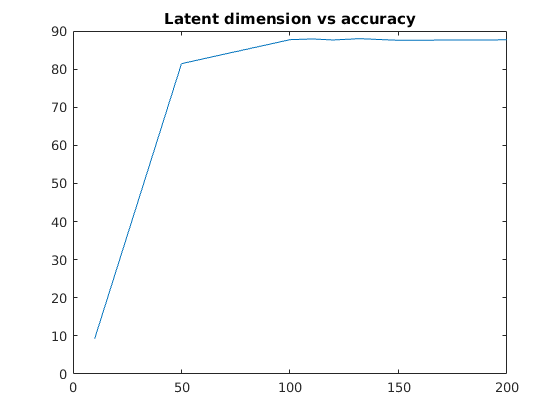
\includegraphics[width=0.8\textwidth]{./images/accuracy.png}
  	\caption{Accuracy vs latent dimension for MNIST}
  	\label{T6}
\end{figure}
The experiments that follow have $k = 133$ fixed. Following is the table showing accuracy of PPCA with missing values and comparision with other variants PCA for handling missing data. 

\newpage

\begin{table}
\begin{center}
\begin{tabular}{ |p{3cm}|p{3cm}|p{3cm}|p{3cm}|  }
 \hline
 Missing Data \% & Accuracy for PPCA with EM & Accuracy for PCA based on Factor Model & Accuracy for PCA based on $\mu$ for missing value\\
 \hline
 \hline
 	0 & 88.01 & 87.97 & 87.97\\
 	1 & 88.25 & 88.27 & 88.40\\ 
	5 & 89.62 & 91.19 & 90.30\\ 
	20 & 92.74 & 93.08 & 93.01\\
	40 & 92.44 & 71.71 & 93.05\\
	60 & 83.49 & 2.81 & 91.44\\
	80 & - & - & 86.31\\
	90 & - & - & 78.08\\
	99 & - & - & 42.94\\
 \hline
\end{tabular}
\end{center}
\caption{Accuracy for Missing data}
\label{Tb1}
\end{table}
	
From table \ref{Tb1}, we can find following observations
\begin{enumerate}
\item The accuracy increase with increase in missing data till a certain fraction. After a threshold the accuracy drops. 
\item The accuracy of PCA handling missing data based on factor model drops significantly (Column 2). The possible explanation for this is that the number of unknowns in the minimization problem $\mathbf{||y-Wx-\mu||}$ becomes large as $x$ is latent and $y$ also has missing data. So the system of equations gives poor estimates of the missing data.
\item PCA based on missing data filled by $\mu$ components show the best acuracy for missing data. A possible explanation is that a large part of data is a background image and digits occupy only lesser fraction. So larger number of missing data are estimated correclty using mean which would be towards background pixel side.
\end{enumerate}

\section{USPS Dataset}
USPS also contains handwritten digit images. The experiment outlined for MNIST is performd again for USPS. For each experiment data is randomly divided into 7 : 3 ratio for training and testing. From figure \ref{T7}, it can be seen tha $k = 100$ is an ideal choice for the latent dimension. Further experiments keep $k=100$. We can also see similar behaviour of this data set as the MNIST. Table \ref{Tb2} also contain the accuracy on conplete data as last column as the data partitioning is random.

\begin{figure}
\centering
  	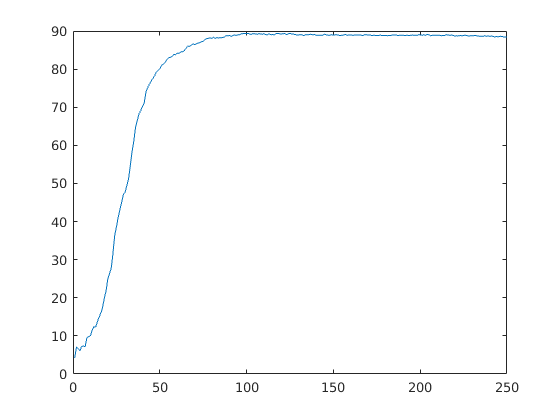
\includegraphics[width=0.8\textwidth]{./images/accuracyUSPS.png}
  	\caption{Accuracy vs latent dimension for USPS}
  	\label{T7}
\end{figure}

\begin{table}
\begin{center}
\begin{tabular}{ |p{3cm}|p{3cm}|p{3cm}|p{3cm}|p{3cm}|  }
 \hline
 Missing Data \% &Accuracy for PPCA with EM & Accuracy for PCA based on Factor Model & Accuracy for PCA based on $\mu$ for missing value & Accuracy Standard PCA on complete data\\
 \hline
 \hline
 	0.5 & 89.96 & 89.57 & 90.12 & 89.42\\
 	1 & 89.93 & 89.72 & 89.84 & 88.84\\ 
	5 & 90.51 & 90.54 & 91.90 & 88.36\\ 
	10 & 91.87 & 91.60 & 93.36 & 89.39\\	
	20 & 92.30 & 92.48 & 93.87 & 90.39 \\
	40 & 83.69 & 84.63 & 91.51 & 88.30\\
	60 & 55.21 & 52.30 & 88.75 & 88.60\\
 \hline
\end{tabular}
\end{center}
\caption{Accuracy for Missing data for USPS}
\label{Tb2}
\end{table}

\newpage

\section{Binary AlphaDigits Dataset}
The data is present in form of $39$ samples for each $36$ classes. Each sample is a $20\times 16$ image. Since the amount of data present is low picking up a large latent dimension is not feasible for calculating the mahalanobis distance. \\\\
From the plot \ref{T8}, it is clear that the accuracy increases till the number of latent dimension $k$ reaches the number of training sample ($k \sim 40$). After that the accuracy does not increase. This makes this dataset difficult to analyse. We donot any further prediction analysis for this dataset. 

\begin{figure}
\centering
  	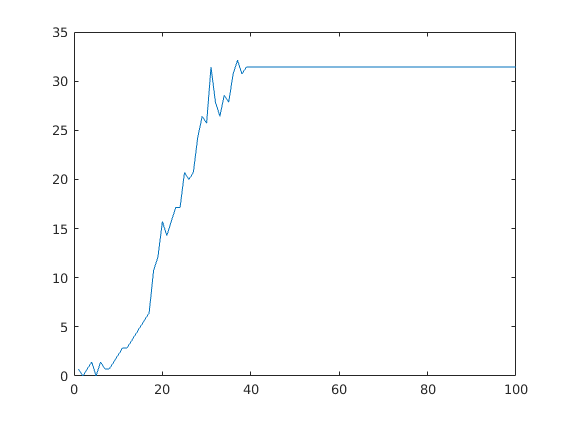
\includegraphics[width=0.8\textwidth]{./images/accuracyAlpha.png}
  	\caption{Accuracy vs latent dimension for Alpha digits}
  	\label{T8}
\end{figure}


